\section{Graph Notions}
\label{sec-preliminary}

In this section, we introduce some basic graph concepts.

\stitle{Graphs}. A {\em weighted undirected graph} (or simply a {\em graph})
is defined as $G (V$, $E$, $w)$, where
(1) $V$ is a finite set of nodes;
(2) $E\subseteq V \times V$ is a finite set of edges, in which $(u, v)$ or $(v, u)$ $\in E$ denotes an undirected edge between nodes $u$ and $v$; and
(3) $w$ is a total weight function that maps each edge in $E$ to a positive rational number.

We simply denote $G (V$, $E$, $w)$ as  $G(V, E)$ when it is clear from the context.

\stitle{Subgraphs}. Graph $H(V_s, E_s,  w_{s})$ is a {\em subgraph} of graph
$G(V$, $E,  w)$ if (1) $V_s \subseteq V$, (2) $E_s \subseteq E$, and (3) $w_{s}(e)$ = $w(e)$ for each edge $e\in E_s$.
%
That is, subgraph $H$ simply contains a subset of nodes and a subset of edges of graph $G$.

We also denote a subgraph $H$ as $G[V_s]$ if $E_s$ is exactly the set of edges appearing in $G$ over the set of nodes $V_s$.


\stitle{Neighbors}. We say that node $v$ is a {\em neighbor} of node $u$ if there exists an edge $(v, u)$ or $(u, v)$ in graph $G$.


\stitle{Paths and cycles}.
A {\em simple path} (or simply a {\em path}) $\rho$ is
a sequence of nodes $v_1/\ldots/v_n$ with no repeated nodes, and, moreover, for each $i\in[1, n-1]$, $(v_i$, $v_{i+1})$ is an edge in $G$.

A {\em simple cycle} (or simply a {\em cycle}) $\rho$ is
a sequence of nodes $v_1/\ldots/v_n$ with $v_1 = v_n$ and no other repeated nodes, and, moreover, for each $i\in[1, n-1]$, $(v_i$, $v_{i+1})$ is an edge in $G$.


The {\em length} of a path or cycle $\rho$ is
the sum of the weights of its constituent edges, \ie $\sum_{i=1}^{n-1} w(v_i, v_{i+1})$.


We also say that a node is {\em reachable} to another one if there exists a path between these two nodes.




\stitle{Shortest paths and distances}.
A {\em shortest path} from one node $u$ to another node $v$, denoted as $\path(u, v)$, is a path whose length is minimum among all the paths from $u$ to $v$.

The {\em shortest distance} between nodes $u$ and $v$, denoted as $\dist(u, v)$, is the shortest length of all paths from $u$ to $v$, \ie
the length of a shortest path from $u$ to $v$.


%%%%%%%%%%%%%%%%%%%%%%%%%%%%%%%%%%%%%%%%%%%%%%%%%%
\begin{figure}[tb!]
%\vspace{-1ex}
\begin{center}
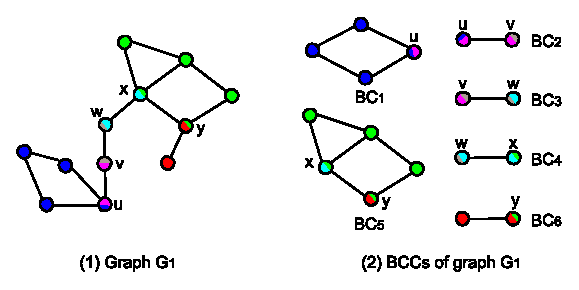
\includegraphics[scale=0.9]{./cut-nodes.eps}
\end{center}
\vspace{-1.5ex}
\caption{Cut-nodes and bi-connected components}
  \label{fig-cut-nodes}\vspace{-2ex}
\end{figure}

\stitle{Connected components}.
A {\em connected component} (or simply a \cc) of a graph is a subgraph in which any two nodes are connected by a path, and is connected to no additional nodes.
A graph is connected if it has exactly one connected component, consisting of the entire graph.


\stitle{Cut-nodes and bi-connected components}.
A {\em cut-node} of a graph is a node whose removal increases the number of connected components in the graph.

A {\em bi-connected component} (or simply a \bc) of a graph is a subgraph consisting of a maximal set of edges such that any two edges in the set must lie on a common simple cycle.

We next illustrate cut-nodes and bi-connected components with an example.

\begin{example}
\label{exm-bccs} Consider graph $G_1$ in Fig.~\ref{fig-cut-nodes}(1), in which labeled nodes $u, v, w, x, y$ are the cut-nodes of $G_1$,
and the corresponding \bccs of $G_1$ are $BC_1, BC_2, BC_3, BC_4, BC_5$, and $BC_6$, and are shown in Fig.~\ref{fig-cut-nodes}(2).
\end{example}